\chapter{Interpretation of Search Results Within Theoretical Models}
\section{Introduction}
It is very often the case that a search for \ac{NP} will yield results
consistent with the currently accepted theory (which, in most particle physics
contexts would be the \ac{SM}). In the absence of a discovery, it is often
desirable to provide additional information in the form of a statistical
interpretation of the results. Such an interpretation typically serves the
following goals:
\begin{itemize}
\item Indicate the strength of the analysis in searching for the proposed model
  or set of models. This can then be used as an objective measure by which to
  rank different analyses or to benchmark the progress of a single analysis as
  data is collected.
\item Falsify, to some confidence level, a particular theory or some region of
  parameter space within that theory. In the case of a reasonably generic model,
  parameterised in such a way that it may represent other theories (or
  approximate their experimental signature), theorists may be able to
  test the predictions of a variety of models directly against the results of
  the interpretation. This will be discussed further in Section~\ref{sec:sms}.
\end{itemize}

Providing an interpretation invariably necessitates some choice of theory or
phenomenological model against which to test the results. The range of theories
will of course depend strongly on the inclusiveness of the experiment. Indeed,
in many cases a single theory will have motivated the analysis in the first
place and the choice of model will be clear. In other cases, the analysis have
been designed to be as inclusive as possible and therefore sensitive to an array
of theories. Typically this is achieved by focussing on a particular detector
signature (for instance missing transverse energy), where a deviation from the
\ac{SM} is a common feature of many \ac{NP} scenarios. Another similar issue
arises when the model being tested is not well defined with a large number of
free parameters which affect the experimental expectations.

\ac{SUSY} searches in particular are subject to these
considerationss. Firstly, as discussed in Section~\ref{sec:susy}, the theory
has a large number of free parameters which may drastically change the
experimental signature. Secondly, whilst a \ac{SUSY} specific interpretation is
possible in principal, it is in some sense not the best use of the experimental
data. The large, multi-dimensional \ac{SUSY} parameter space and corresponding
variation in the physics signatures necessitates an inclusive analysis
strategy - typically looking for high jet multiplicities in association with
large missing transverse energy. Such signatures may occur in a variety of
potential \ac{NP} theories. With an appropriate interpretation, the results of
an inclusive \ac{SUSY} search can be used to draw conclusions about these
theories, restricting their parameter space or ruling them out altogether.

\ac{SUSY} searches at the \ac{LHC} have typically provided two
interpretations. The first, within a very restricted class of \ac{SUSY} theoreis
known as \ac{mSUGRA}. The second, within one or more so-called ``Simplified
Models'', chosen by theorists to represent a wide range of possible \ac{NP}
theories, categorised according to their phenomenological properties.

\section{Models}
\subsection{\acl{mSUGRA}}

\subsection{Simplified Models}
\label{sec:sms}
It is often the case that theorists, having devised some theory, and made
concrete phenomenological predictions from it, wish to test it against
experimental data. The difficulty then arises of taking these predictions and
translating them into a form where they can be compared directly with
experimental results. Typically, these results will be provided in the form of
one or more event yields, corresponding background predictions and statistical
and systematic uncertainties. In some (but probably not most) cases, the
relevant correlations will also be included. The theorist must then take the
predictions of the theory and apply experimental resolution effects to them in
order to simulate the expected signal yield. Modern detectors are highly complex
and require very complex simulation to precisely model all of the resolution
and acceptance effects. In some cases, in particular for relatively simple
kinematic quantities, a simplified parameterisation may suffice but detailed
checks will be required to confirm that a given approximation reproduces, with
adequate fidelity the full detector simulation or the actual recorded data. If
it can be confirmed that this is the case, the theorist may then proceed to redo
the work of the experimentalist in modelling the various statistical and
systematic effects in the form of a likelihood function. Finally, they may then
utilise all of these components to produce their own statistical interpretation
of the data against the chosen theory.

Clearly, this procedure is both laborious and error-prone. It was therefore
proposed that the \ac{LHC} experiments would provide a richer interpretation in
the context of a set of ``Simplified Models''. Broadly speaking, a simplified
model is a highly simplifed effective theory, chosen to characterise a
particular phenomological scenario present within one or more \ac{NP}
models. Free parameters which have little effect on the physics are integrated
out, leaving only those with a large effect on the physics. In constructing a
number of these models, the full space of possibly physical signatures arising
in much more complicated theories may be spanned.

Although the concept of a simplified model is quite general, the discussion here
will focus on those inspired by \ac{SUSY} or ``\ac{SUSY}-like'' theories, and
more specifically those relevant to the single-leptonic experimental search
described in previous chapters.

% \todo[size=\tiny, linespacing=0.5]{Mention that SMS are used for characterisation of discovery as well as
%   design of searches}

\subsubsection{Dark Matter Models}


\section{Statistical Background}

\section{New Physics Models}
\section{Results}
Waay
\begin{figure}
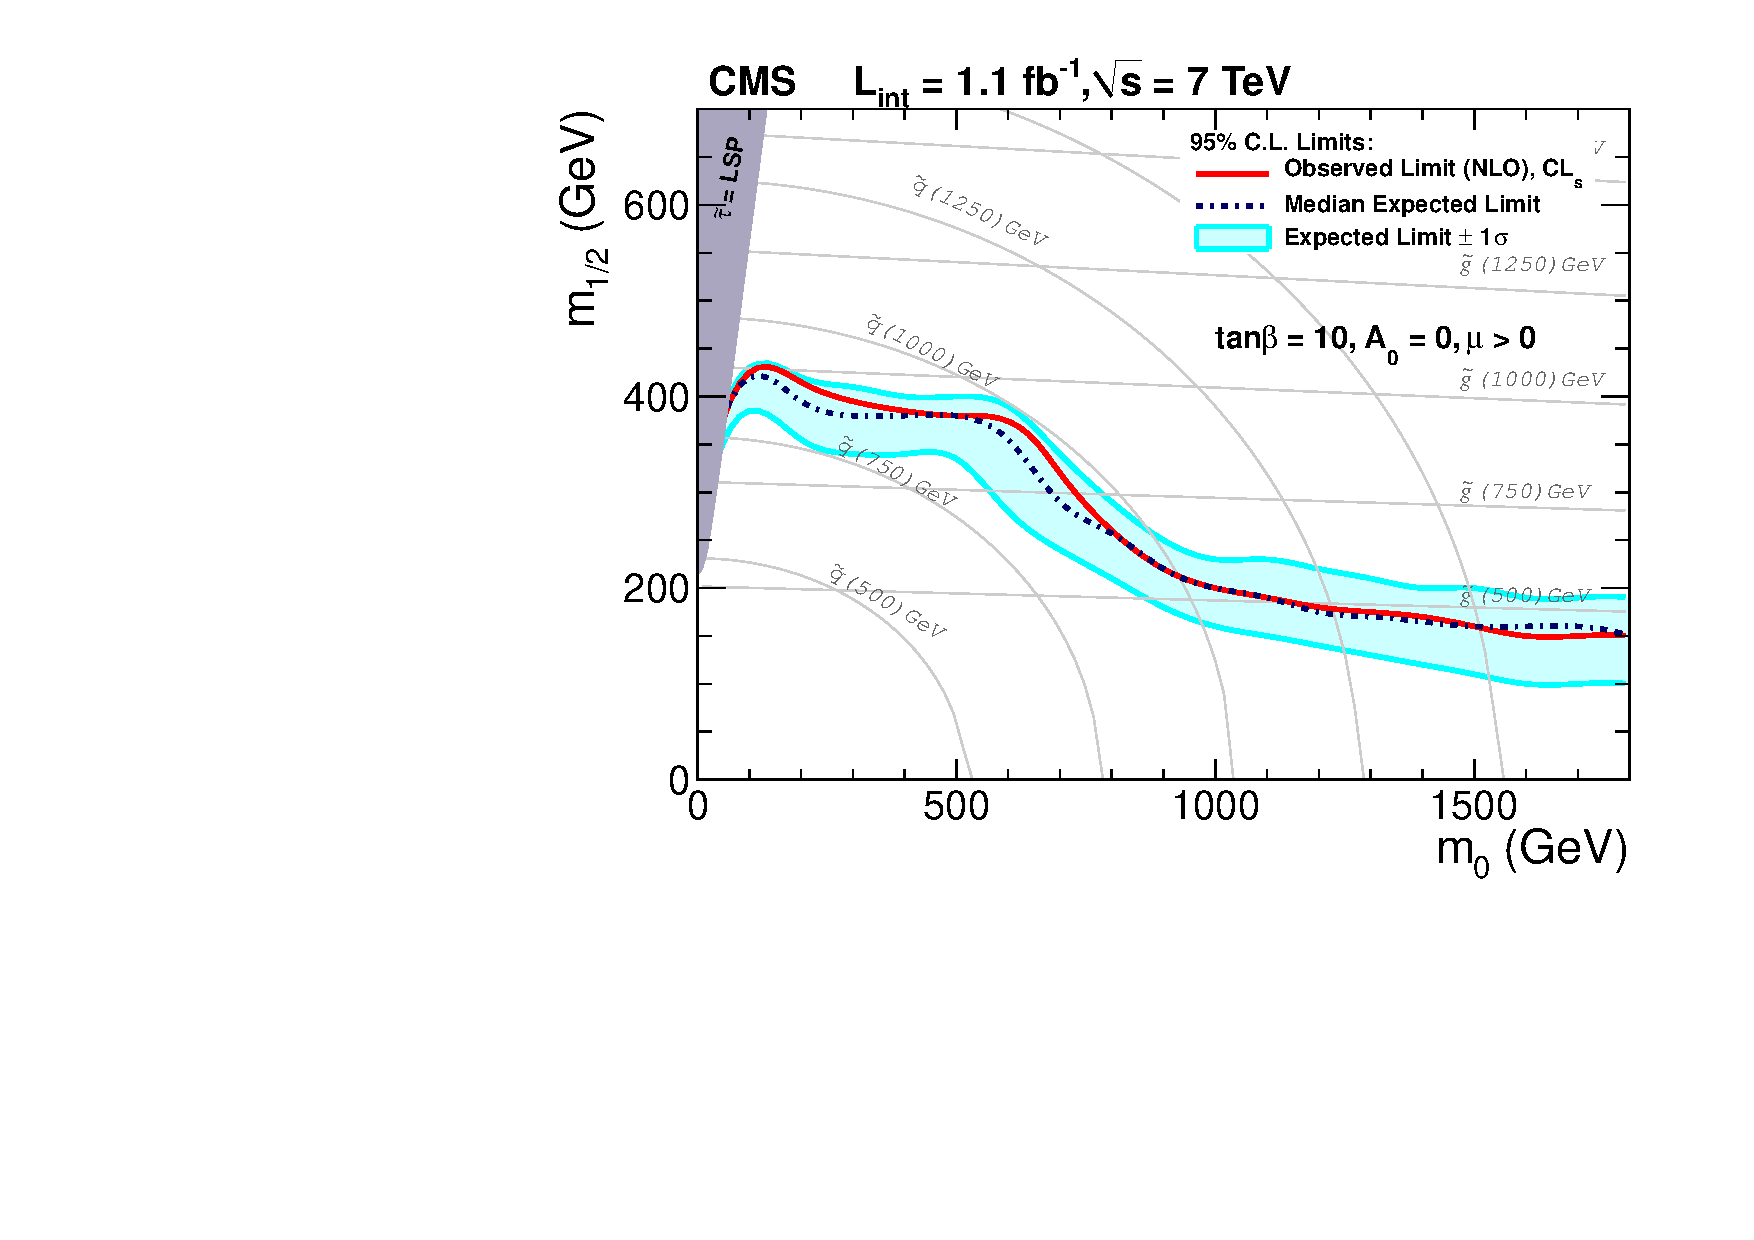
\includegraphics[width=\textwidth]{fig/RA4_ExclusionLimit_tanb10}
\end{figure}